\clearpage{}
\section{Discuss tactics to achieve modifiability, performance, security,
reliability, robustness, usability.}

Requirements: functional and \textbf{non-functional quality attributes}.

\subsection{Modifiability}

$\rightarrow$ Design must be easy to change.

The goal is to minimize the number of software units requiring changes.
Two tactics:
\begin{itemize}

    \item \textbf{Directly affected}: responsibilities change (cluster
        anticipated changes)

        \begin{itemize}
            \item Anticipate expected changes: encapsulate each anticipated change in one unit
            \item Cohesion: all pieces, data, and functionality of each unit contribute to its purpose
                and responsibilities
            \item Generality: accommodate change by modifying a unit's inputs rather than modifying
                the unit itself
        \end{itemize}

    \item \textbf{Indirectly affected}: only implementation changes
        (reduce dependencies)

        \begin{itemize}
            \item Coupling: reduce the degree to which a unit depends on another
            \item Interfaces: interact with other units only through their specified interface
            \item Multiple interfaces: provide a new interface for new data or services (preserving
                existing interfaces)
        \end{itemize}
\end{itemize}


\subsection{Performance}

$\rightarrow$ Constraints on system speed and capacity (response time, throughput, load).
Following tactics can be used:
\begin{itemize}
	\item Increase resources
	\item Improve utilization of resources (e.g:
        concurrency/parallelization)
	\item Improve allocation of resources (scheduling)
	\item Reduce demand for resources (increase efficiency)
\end{itemize}


\subsection{Security}
$\rightarrow$ Controlling access to resources. Two tactics:

\begin{itemize}
    \item \textbf{Immunity (preventing an attack)}: risk avoidance
        \begin{itemize}
            \item Ensure that all security features are included
            \item Minimize exploitable security weaknesses
        \end{itemize}

    \item \textbf{Resilience (recovering from an attack)}: risk
        acceptance
        \begin{itemize}
            \item Segment the functionality to contain attack
            \item Enable the system to quickly restore functionality
        \end{itemize}
\end{itemize}

\subsection{Reliability Vs Robustness}
\subsubsection{Reliability}

$\rightarrow$ Performing correctly \textcolor{red!80!black}{under assumed conditions}. (Fault is a
defect in a product). System correct = 100\% reliable.

\begin{figure}[!ht]
    \centering
    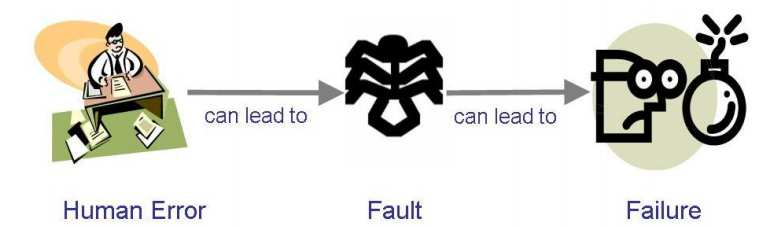
\includegraphics[width=0.6\linewidth]{reliability.png}
    \caption{Error-Fault-Failure}
\end{figure}

Two kinds of tactics:

\begin{itemize}
    \item Preventing faults: by writing well the code and avoiding human error.
    \item Tolerating faults: Fault detection, identification and
        \textbf{recovery} (FDIR). 

        Two kind of detection, active (look for symptoms) vs.\ passive (wait fault).
\end{itemize}

\subsubsection{Robustness}

$\rightarrow$ Performing correctly \textcolor{red!80!black}{under adverse conditions}.
Safe = free from unacceptable behaviours.

\begin{itemize}
    \item Defensive design: anticipate external problems
    \item Mutual suspicion: check inputs for correctness, consistency, pre-conditions
    \item Redundant calculations (ex: space shuttle, radiation glitch)
    \item State recovery tactics (same as for reliability)
\end{itemize}

\subsubsection{Recovery tactics}

Both robustness and reliability can use the following technics to recover from undesirable
state:

\begin{itemize}
    \item Undoing transaction (ex: database)
    \item Checkpoint / rollback (saved state)
    \item Backup
    \item Degraded service (provide an older stable version)
    \item Correct and continue (fix the symptoms)
    \item Report (returns to previous state and record the problem)
\end{itemize}

\subsection{Usability}
$\rightarrow$ Ease of use of the system.
Tactics at architectural level:
\begin{itemize}
    \item UI should be in its own software unit/layer
    \item Need a UI event handler process
    \item Support for UI functionality cancel/undo, views,\ldots
    \item Maintain a model of its environment Mme, industrial process
\end{itemize}
